\chapter{Introduction}
\label{chapter:introduction}

Pressure ulcers (which are also known as decubitus ulcers or bed sores) are a major problem in health care due to high prevalence and high cost of treatment. Some ulcers do not heal for decades. If not properly managed, pressure ulcers may cause complications such as septicemia or even death. Early prevention of pressure ulcers is beneficial over curing. 
\begin{figure*}
    \vspace{-0.7cm}
      \centering
      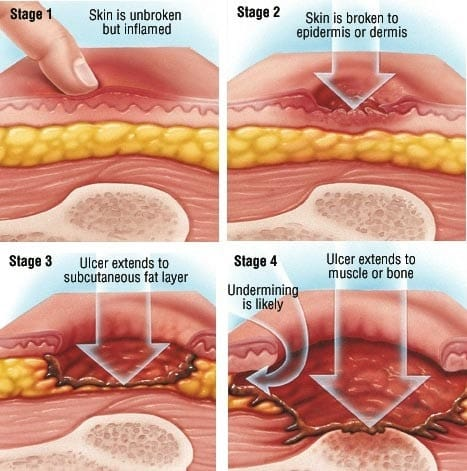
\includegraphics[width=0.5\textwidth]{figs/pressure-sore-stages.jpg}
      \vspace{-0.2cm}
      \caption[Stages of a pressure ulcer]{Stages I-IV of pressure ulcers according to NPUAP classifications. Image credits: https://www.nursinghomelawcenter.org/bed-sore-pictures.html}
      \label{fig:pustages}
\vspace{1.0cm}
\end{figure*}

\section{Literature Review}
Prolonged external pressure into bony areas of body causes pressure ulcers in bed-ridden patients. Prevailing patho-physiological understanding of pressure ulceration is very incomplete. Several existing theories suggest that reduction of oxygen supply (under external pressure) to skin tissues causes cell death through an ischaemia-reperfusion cycle, which results in pressure ulcer formation. Another theory suggests that internal pressure on muscle tissues by bones causes ulceration. None of these theories are empirically verified. Ischaemia reperfusion models describe ulceration as a phenomenon starts at the skin and spread deep where as the last theory describe it as a phenomenon starts at muscle tissues closer the bones and spreads in the opposite direction towards bones. 

Reswick and Rogers studied effect of pressure and time on cell death in 1976 modelling ischaemia oriented theory. There is no considerable improvement since then other than a few papers suggesting slight modifications. Few experiments that were ever conducted on reperfusion theory also provide inconclusive values. There is no satisfactory empirical research on internal pressure theory, although Deep Tissue Injury (DTI), a recently defined category of pressure ulcers, is specifically and widely believed to be a result of internal pressure from bones. 
\begin{figure*}[t]
    \vspace{-0.7cm}
      \centering
      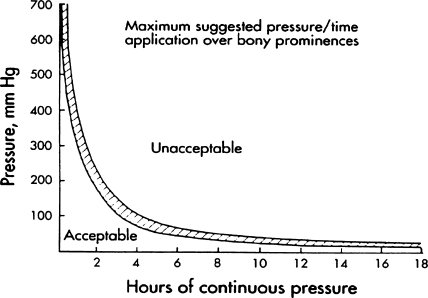
\includegraphics[width=0.7\textwidth]{figs/reswick_rojers.jpg}
      \vspace{-0.2cm}
      \caption[Reswick Rogers Experiment]{Reswick and Rogers' pressure time cell threshold graph.}
      \label{fig:reswickrogers}
\vspace{1.0cm}
\end{figure*}

Exact bio-mechanical impact of pressure on human body (skin and muscles) is not yet known given that only a few unsatisfactory bio-mechanical models from early research based on animal testing and qualitative speculations without quantitative data are available. There is no sufficient data on the mechanism through which external pressure causes an ischemia-reperfusion cycle. Furthermore, there is no quantitative empirical evidence for the effect of other proposed bio-mechanical factors such as shear, friction and moisture also. 

Pressure ulcers are usually located in specific sites of the body such as back of head, shoulders, buttocks,  knees, elbows, hips and heels. \begin{figure*}[t]
    \vspace{-0.7cm}
      \centering
      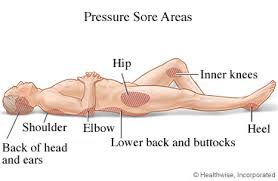
\includegraphics[width=0.5\textwidth]{figs/ulceration-points.jpg}
      \vspace{-0.2cm}
      \caption[Ulceration points]{Common sites where ulceration occurs.}
      \label{fig:ulcerpoints}
\vspace{1.0cm}
\end{figure*} Pressure ulcers occur in four stages according to NPUAP staging system and there are specific guideline for treatment and each stage. There is no empirical data available on how these factors affect different parts of body and different type of bodies. No empirical data is available on how the healing rates or reulceration (reulceration is not prominent as in the case of diabetic foot ulceration) was affected by the pressure. 

\subsection{Pressure Ulcer Prevention}
The main pressure ulcer prevention strategy which is strongly recommended by health care authorities is frequent patient repositioning. This strategy was popularized after the end of World War II by Ludwig Guttmann, based on face validity. Caretakers should turn the patients into a different sleeping posture for every 2 h (This duration was Guttmann's ad hoc recommendation). 

The absence of high quality research evidence supporting the efficacy of repositioning was discussed in a Cochrane systematic review published in 2014 (and updated in 2020). Research does not show significant advantage of 2 h repositioning over alternative time periods or no-repositioning. Currently available data are low certain and not sufficiently reliable to provide a conclusion. Existing studies do not consider bio-mechanical facts explicitly. Recently some researchers castigated the repositioning strategy for side effects such as disturbance to sleeping patterns, negative impact on dementia patients and back pain of caretakers. Recently NICE guidelines increased the time period from 2 h to 6 h for normal patients and 4 h for patients in high-risk category. Standard guidlines do not recommend to alter repositioning plans according to existing ulcers and there are no research ever conducted in that area. The efficacy of other proposed prevention strategies including the use of pressure redistribution surfaces also are not supported with research, contrary to the availability of wide range of products in the market.

\subsection{Personal Risk Assessment and Documentation}
There are several patient risk assessment indicators including Braden and Waterlow scales. The importance of a systematic scale for risk assessment is often emphasized over using clinical judgement alone. Clinical evidence on the efficacy of these tools is still insufficient and uncertain.
Proper documentation is of crucial importance in modern health care. There are several paper-based or electronic documentation systems for pressure ulcers. According to studies, the purpose of existing documentation systems is not met with ulcer prevention and care. The patient repositioning plans are rarely documented. There are no records of bio-mechanical data. Existing electronic documentation systems are desktop applications that store records inside a single end-user device. The recent advancement of mobile, web, IOT and cloud technologies are not yet employed for pressure ulcer documentation. 

\section{Requirement of A Health Information System}
Ajami and Khalegi discussed the importance of a wireless sensor network for pressure monitoring. There is need for a sophisticated Health Information System (HIS) that supports not only remote pressure monitoring and electronic documentation but also important utilities to optimize care plan such as posture detection, ulceration point (the specific areas of body which are more prone to ulceration) detection, pressure/risk estimation, repositioning schedule calculation and carer notification. Although there are several implementations addressing subsets of above tasks already, constructing a health information system in a holistic point of view is a novel concern. Such information system should network patients, caretakers, guardians and doctors together and generate, collect, store, analyse and interpret data for better care planning. Considering the fact that pressure ulcer is a grey area of medical research the information system should work as tool to investigate bio-mechanical and clinical details of bed-ridden patients. Another requirement is to provide support for semi-automation of patient care through care plan optimization like reposition schedule calculation and carer notification system. Wide availability of mobile technology paves a way for a flexible and more sophisticated reporting system. Integrating low cost pressure sensing equipment to the information system provides opportunity to monitor and collect data for long periods and to widen the scope of research including the majority of ulcer-prone patients that reside in household settings. Reduction of cost will facilitate research into pressure ulcers in developing countries.

\section{Previous Research}
There are several research into pressure monitoring equipment for bed-ridden patients. Most of those research are based on pressure measurement posture detection and pressure image segmentation. Some research considered automatic patient repositioning by actuators. The contribution of the researchers of University of Dallas has considered a wide range of aspects that are related to pressure ulceration phenomenon. These researchers paid attention to the biomechanics of pressure ulceration. But this is prior to 2014, the year several systematic reviews were published questioning the efficacy of prevention methods. Therefore the limitations to their study is not apparent in their original papers. They purposively conflate data related to different theories, scenarios and settings to achieve final results. Therefore their results are considerably depended on ad-hoc assumptions and speculations from indirect data. In this research we adopted some of their results for our purpose as the best solution available carefully evaluating the limitations.


